\documentclass[10pt]{article}
\usepackage[margin=0.82in]{geometry}
\usepackage{amsmath,amssymb,graphicx}
\usepackage[numbers,sort&compress]{natbib}
\usepackage{url}
\graphicspath{{../results/}{../results/paper_scaling/}{../results/frontier/}{../results/mechanism/}{../results/heldout/}{../results/systems/}{../results/reviewer_controls/}}
\renewcommand{\bibfont}{\small}

\title{SplitMoE: Partial-Width Shared Capacity for Parameter-Efficient\\Sparse Mixture-of-Experts Language Models}
\author{Priyanshu Maurya\\Independent Researcher}
\date{}

\begin{document}
\maketitle

\begin{abstract}
Conventional sparse mixture-of-experts (MoE) layers store every expert as a complete feed-forward network, even though some transformations may be useful across routes. SplitMoE instead gives every token a small shared branch plus routed private branches: common capacity is stored once, while private capacity remains conditional. In an eight-layer, eight-expert Top-1 language model trained for 213M token positions, a 25/75 shared/private split uses 16.4\% fewer total parameters than Standard MoE at equal activated capacity. Across three paired seeds, SplitMoE lowers validation loss by $0.05611$ at output scale 1 and $0.03569$ at scale $1/\sqrt{2}$; both 95\% confidence intervals exclude zero. At equal total storage, it lowers loss by $0.06261$ while activating 6.3\% more parameters. The benefit is not universal: with 16 experts and Top-4 routing, a conventional full shared expert performs best. Route interventions and width-matched similarity measurements indicate that SplitMoE's private branches are route-dependent and less output-redundant. These results support SplitMoE as a regime-dependent parameter-allocation strategy, not a universally superior MoE.
\end{abstract}

\section{Introduction}
Sparse MoEs route each token through a small subset of feed-forward experts, decoupling stored parameters from per-token activation \citep{shazeer2017outrageously,lepikhin2020gshard,fedus2022switch}. The usual layer stores $N$ independent expert functions,
\begin{equation}
F_{\mathrm{standard}}(x)=\sum_{i\in\operatorname{TopK}(x)}p_i(x)E_i(x).
\end{equation}
This conditional capacity is useful, but complete independence is not free: experts in one layer may separately store and learn transformations needed by many routes.

We ask whether the active transformation can instead be represented as common capacity plus conditional specialization. Let
\begin{equation}
E_i(x)=S(x)+P_i(x),
\end{equation}
where $S$ is shared within a layer and $P_i$ is private. For normalized routing weights, the corresponding computation is
\begin{equation}
F_{\mathrm{split}}(x)=S(x)+\sum_{i\in\operatorname{TopK}(x)}p_i(x)P_i(x).
\label{eq:split}
\end{equation}
The shared computation is stored and evaluated once. The router selects residual specialization after shared capacity is supplied.

Always-active shared experts are established in DeepSeekMoE and Qwen1.5-MoE \citep{dai2024deepseekmoe,qwen2024moe}. Our question is narrower: what happens when a fixed active FFN budget is explicitly divided between a \emph{partial-width} shared branch and partial-width private branches? We evaluate this allocation under matched activated capacity, matched storage, different shared fractions, different routing regimes, causal expert interventions, and width-controlled representation analysis.

Our findings are deliberately conditional. Partial-width sharing moves the observed parameter-quality frontier under Top-1. Under Top-4, it offers a storage/quality tradeoff, while a full shared expert is strongest at matched FFN storage and activation. This regime dependence is itself useful: it separates evidence for reusable capacity from a claim that one allocation is always optimal.

\section{Related Work}
Modern sparse language-model MoEs build on sparsely gated expert layers \citep{shazeer2017outrageously}, scalable Top-$K$ routing \citep{lepikhin2020gshard}, simplified Top-1 routing \citep{fedus2022switch}, and stability methods such as router z-loss \citep{zoph2022stmoe}. These routing and balancing techniques are controls in this work, not contributions.

DeepSeekMoE introduced fine-grained segmentation and shared-expert isolation to capture common knowledge and reduce routed-expert redundancy \citep{dai2024deepseekmoe}; Qwen1.5-MoE subsequently used shared and routed experts in a released model \citep{qwen2024moe}. SplitMoE differs by allocating a controlled fraction of a target active width to one partial-width shared FFN and the remainder to partial-width routed FFNs, then studying the resulting storage frontier. Our full shared-expert control directly tests whether partial-width decomposition improves over the established design.

Low-rank and shared-base work provides a second close line of precedent. StructMoE augments experts with dynamically selected low-rank components \citep{sarwar2024structmoe}. DeRS represents upcycled experts using a shared base and sparse or low-rank deltas \citep{huang2025ders}. D$^2$-MoE and PARSER decompose pretrained expert matrices into shared bases and compressed residuals \citep{gu2025d2moe,jung2026parser}. These works make broad novelty claims about ``shared plus private'' untenable. Our contribution instead lies in from-scratch partial-width FFNs and the controlled empirical evidence: allocation sweeps, paired seeds, causal private-route tests, and same-width output-redundancy controls.

\section{Method}
\subsection{Architecture}
Each FFN is a SwiGLU network with hidden width $w$. Standard MoE stores $N$ width-$D$ experts and activates $K$:
\begin{equation}
W_{\mathrm{store}}^{\mathrm{standard}}=ND,
\qquad
W_{\mathrm{active}}^{\mathrm{standard}}=KD.
\end{equation}
SplitMoE stores one shared width $sD$ and $N$ private networks of width $(1-s)D$:
\begin{equation}
W_{\mathrm{store}}^{\mathrm{split}}=sD+N(1-s)D,
\qquad
W_{\mathrm{active}}^{\mathrm{split}}=sD+K(1-s)D.
\end{equation}
For Top-1, the latter equals $D$ for every $s$. For $K>1$, a fixed split reduces active capacity unless private width is increased; we therefore include a separate equal-active control.

\begin{figure}[t]
\centering
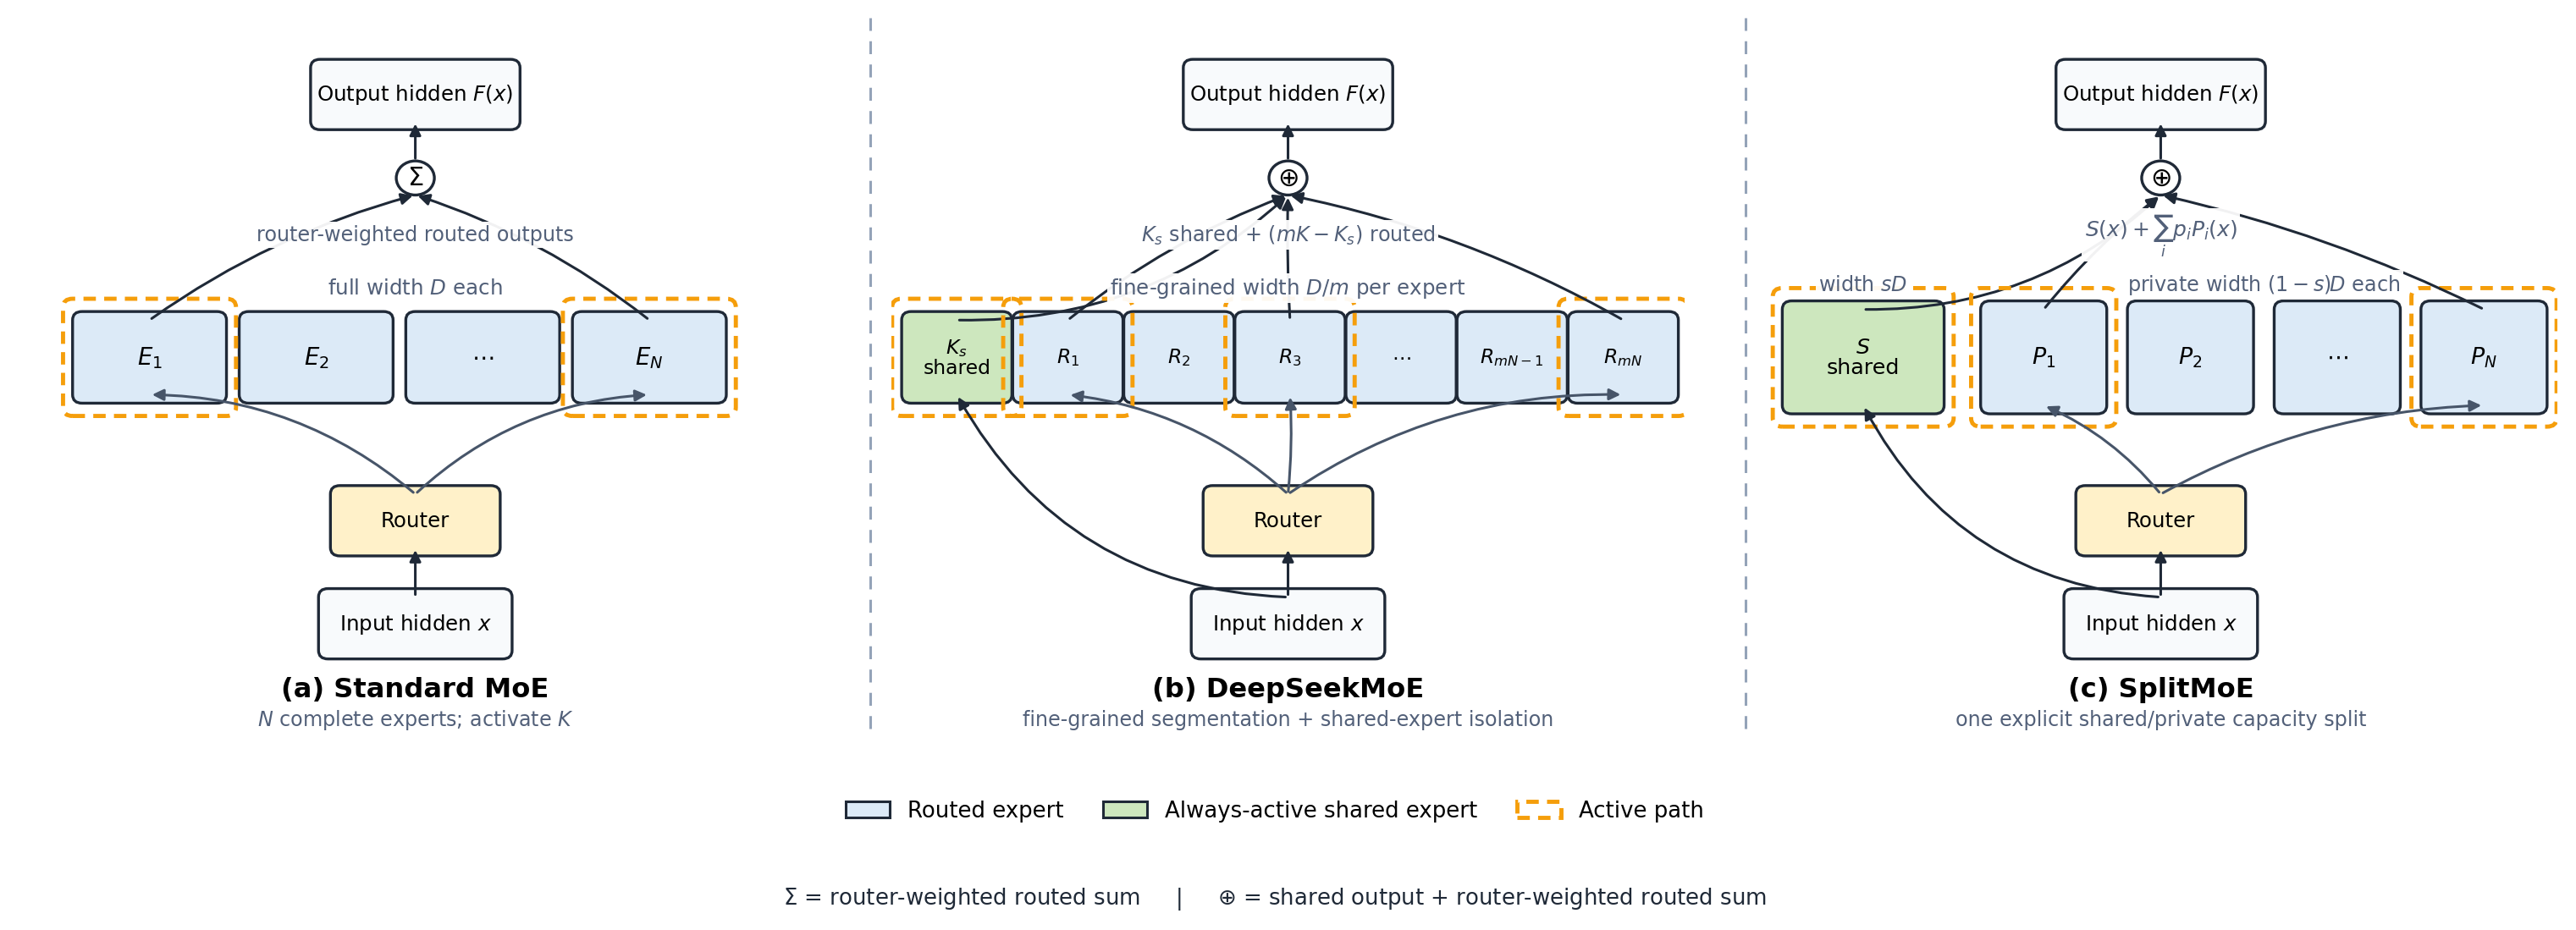
\includegraphics[width=.88\linewidth]{architecture.png}
\caption{Standard MoE stores complete independent experts. SplitMoE supplies each token with one shared partial-width FFN plus routed private partial-width FFNs.}
\label{fig:architecture}
\end{figure}

The implementation adds shared and routed outputs, then applies an output multiplier $\alpha$. Initial experiments use $\alpha=1/\sqrt{2}$; the reviewer control tests both $\alpha=1$ and $1/\sqrt{2}$ for Standard and Split. Top-1 experiments use straight-through router scaling: forward expert weight is one while router gradients follow the selected probability. Top-4 experiments renormalize selected probabilities. All experiments add a load-balancing auxiliary loss with coefficient 0.01 and router z-loss with coefficient 0.001.

\subsection{Controls}
We distinguish four matching rules. (1) \emph{Equal active width}: Standard-1024 versus Split-25 (256 shared + 768 private) under Top-1. (2) \emph{Equal total storage}: Standard-640 versus Split-50 in the small model, and Standard-800 versus Split-25 in the all-MoE model. (3) \emph{Practical Top-4}: shared 256 + private 768, reducing storage and activation. (4) \emph{Equal-active Top-4}: shared 256 + four private routes of width 960, since $256+4(960)=4(1024)$. We also compare one always-active width-1024 expert plus 15 routed width-1024 experts with Top-3 routing; this matches the Standard-16E Top-4 FFN storage and activation up to a negligible router-size difference. A proposed control with two private partial-width branches is not a distinct architecture here: concatenating their SwiGLU hidden units exactly recovers one wider private SwiGLU expert when both branches are routed together.

\section{Experimental Setup}
Models are decoder-only Transformers with SwiGLU FFNs, RMSNorm, learned positional embeddings, context 256, and the 49,152-token SmolLM2 tokenizer. The main scaling models have eight layers, width 512, eight attention heads, and an MoE in every layer. The initial comparison trains from scratch for 6,500 optimizer steps with effective batch 64 (106.5M token positions). The output-scale factorial uses the same optimizer schedule on two T4 GPUs with effective batch 128 (213.0M token positions). Results from these two token budgets are reported separately. Both use AdamW, peak learning rate $3\times10^{-4}$, 500 warmup steps, FP16, and paired seeds 1337, 2027, and 3407.

The pretraining mixture contains up to 100,000 packed blocks from each of TinyStories, WikiText-103, CodeParrot Clean, and OpenWebMath. A deterministic hash assigns one percent of documents to validation; reported in-domain validation uses an identical fixed domain-balanced sample across paired models. The smaller allocation sweep uses eight layers with MoE layers 2, 4, 6, and 8 and five paired seeds for 10,000 steps.

External evaluation uses the pinned 5,153-example English LAMBADA test split \citep{paperno2016lambada}, which was not intentionally included in the training mixture. Because the original training corpus was not deduplicated against LAMBADA, we do not call it contamination-free. Each document is tokenized independently without special tokens. We retain the final 257 tokens for overlength documents and batch equal lengths without padding or cross-document context. All checkpoints use one CPU FP32 evaluation path. Full-token autoregressive loss is primary; final-word token loss and exact argmax token-sequence match are teacher-forced diagnostics, not free-running generation accuracy.

We treat training seeds, not validation checkpoints, as independent samples. Intervals are two-sided Student's $t$ intervals over paired seed differences. A confidence interval crossing zero is not interpreted as equivalence. Before the Top-4 equal-active control, we fixed a non-inferiority margin of 0.01 LM loss; the upper confidence endpoint must lie below it.

\section{Results}
\subsection{Top-1 parameter frontier}
The small-model allocation sweep indicates that private capacity remains important. Among tested ratios, Split-25 gives the best observed validation-loss/storage tradeoff: it stores 18.75\% fewer parameters inside replaced MoE FFNs than Standard-1024 and has a paired difference of $-0.00138$ with 95\% CI $[-0.00604,+0.00328]$. This is no detected degradation, not proof of equivalence. At exactly equal total model storage, Split-50 beats Standard-640 in all five seeds by $-0.01437$ $[-0.01982,-0.00893]$, although Split activates 5.4\% more full-model parameters.

\begin{figure}[t]
\centering
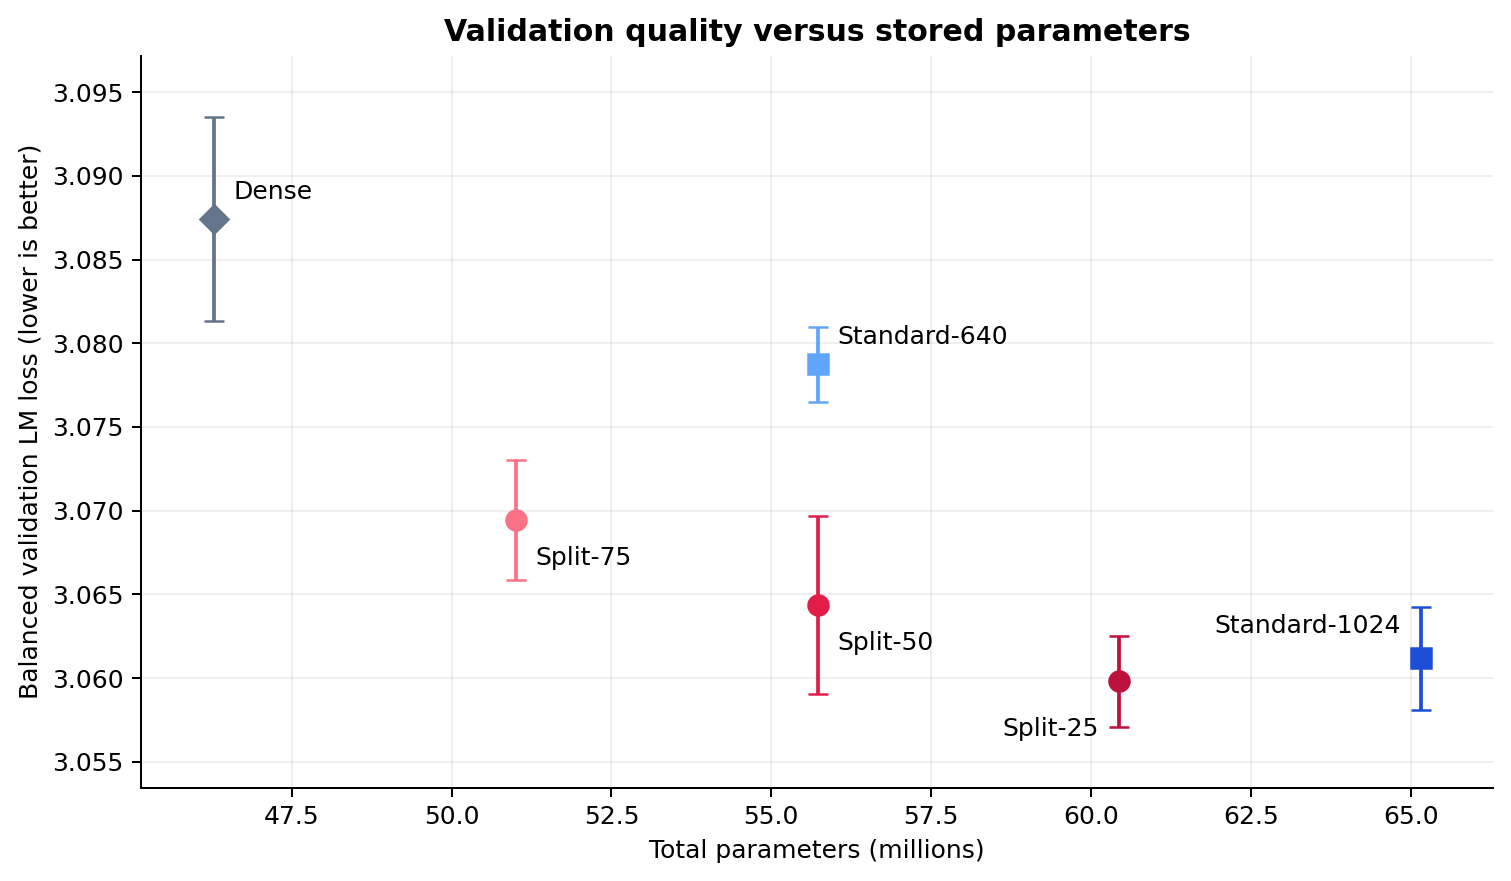
\includegraphics[width=.72\linewidth]{quality_vs_parameters.png}
\caption{Five-seed small-model validation quality versus total stored parameters. Error bars are two-sided 95\% Student's $t$ intervals over training seeds.}
\label{fig:frontier}
\end{figure}

The initial all-MoE Top-1 comparison strengthens the result (Table~\ref{tab:top1}). Split-25 reduces total storage by 16.4\% at matched activation and wins every paired seed and domain. These runs used effective batch 64 and 106.5M token positions. Their larger improvement relative to the small-model sweep is not presented as a scaling law because MoE placement and training horizon also differ.

\begin{table}[t]
\centering
\caption{Initial eight-expert Top-1 all-MoE results at effective batch 64 and 106.5M token positions (mean over three seeds).}
\label{tab:top1}
\begin{tabular}{lrrr}
\hline
Model & Total params & Active/token & Validation loss \\
\hline
Standard & 134.39M & 46.31M & 3.34034 \\
Split-25 & \textbf{112.37M} & 46.31M & \textbf{3.25393} \\
\hline
\end{tabular}
\end{table}

We then isolate the branch-output multiplier in a batch-matched $2\times2$ factorial (Table~\ref{tab:scale}). At scale 1, Split-25 beats Standard-1024 by $-0.05611$ with paired 95\% CI $[-0.07734,-0.03488]$; at scale $1/\sqrt{2}$, it wins by $-0.03569$ $[-0.05273,-0.01865]$. Split changes by only $+0.00069$ $[-0.00389,+0.00528]$ between the two scales, whereas Standard improves by $-0.02111$ when scaled by $1/\sqrt{2}$. The difference-in-differences is $-0.02042$ $[-0.02745,-0.01339]$, so scale affects the architectures differently, but it does not explain Split's advantage at either tested value.

\begin{table}[t]
\centering
\caption{Batch-matched Top-1 output-scale controls at effective batch 128 and 213.0M token positions (mean over three paired seeds).}
\label{tab:scale}
\begin{tabular}{llrrr}
\hline
Model & Scale $\alpha$ & Total params & Active/token & Validation loss \\
\hline
Standard-1024 & $1$ & 134.39M & 46.31M & 3.08106 \\
Standard-1024 & $1/\sqrt{2}$ & 134.39M & 46.31M & 3.05994 \\
Split-25 & $1$ & \textbf{112.37M} & 46.31M & \textbf{3.02495} \\
Split-25 & $1/\sqrt{2}$ & \textbf{112.37M} & 46.31M & \textbf{3.02425} \\
Standard-800 & $1$ & 112.37M & \textbf{43.56M} & 3.08756 \\
\hline
\end{tabular}
\end{table}

At exactly equal total storage and scale 1, Split-25 beats Standard-800 in all three seeds. The paired difference is $-0.06261$, with 95\% CI $[-0.06340,-0.06183]$. Split activates 6.3\% more full-model parameters, so this is an equal-storage comparison, not an equal-compute comparison. A nominal two-private-branch control is algebraically identical to Standard-1024 in this implementation: concatenating equally routed SwiGLU hidden units produces the same function class as one wider SwiGLU expert.

\begin{figure}[t]
\centering
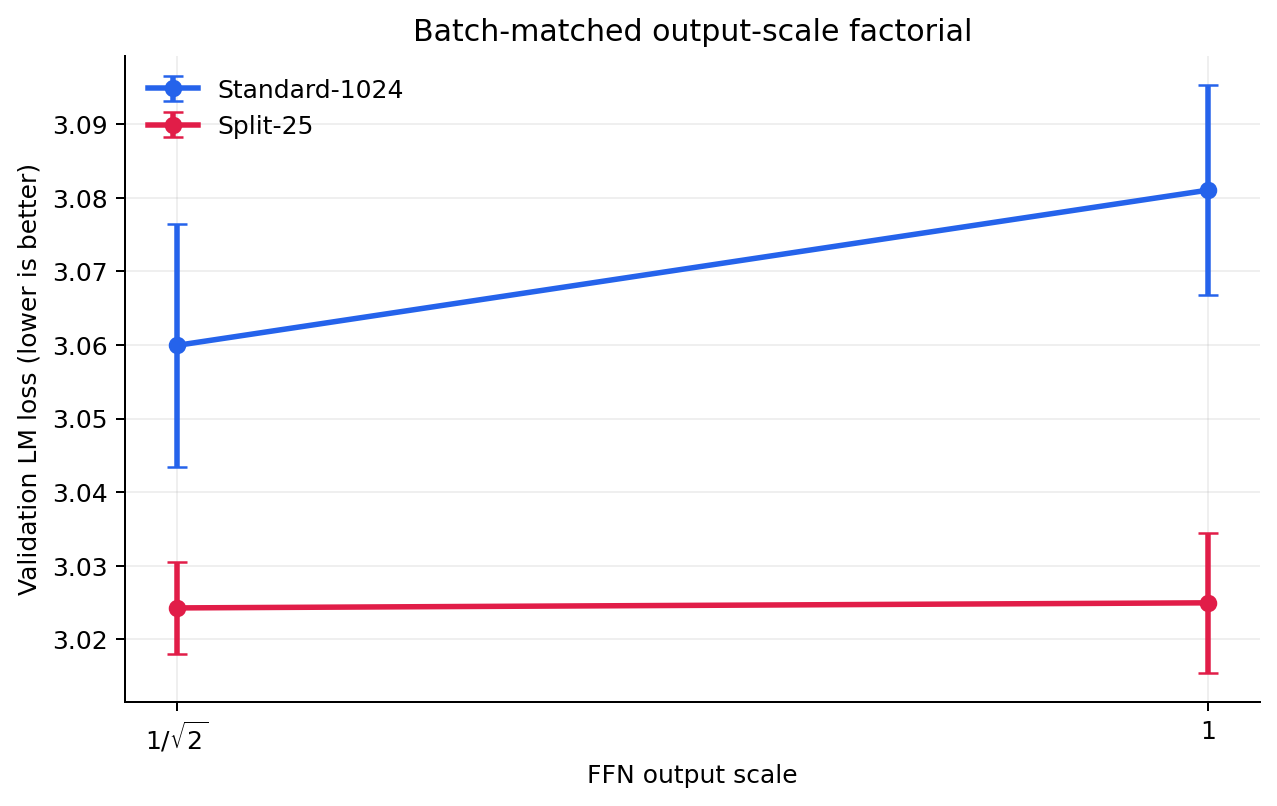
\includegraphics[width=.72\linewidth]{output_scale_factorial.png}
\caption{Batch-matched output-scale factorial. Points show three-seed means; error bars are two-sided 95\% Student's $t$ intervals over seeds. Split-25 remains better at both tested scales.}
\label{fig:scale}
\end{figure}

\subsection{Top-4 regime}
Table~\ref{tab:top4} separates practical storage reduction from equal-active comparison. Practical Split saves 20.1\% total parameters and 11.2\% activated parameters, with a paired loss difference of $+0.01362$ $[-0.00725,+0.03448]$. Equal-active Split recovers most of this observed deficit: $+0.00053$ $[-0.01815,+0.01921]$ relative to Standard. Its upper endpoint exceeds the preregistered $+0.01$ margin, so non-inferiority is not established.

\begin{table}[t]
\centering
\caption{Sixteen-expert Top-4 results (mean over three paired seeds).}
\label{tab:top4}
\begin{tabular}{lrrr}
\hline
Model & Total params & Active/token & Validation loss \\
\hline
Standard & 235.09M & 84.09M & 3.11376 \\
Practical Split & \textbf{187.90M} & \textbf{74.65M} & 3.12738 \\
Equal-active Split & 225.65M & 84.09M & 3.11430 \\
Full shared expert & 235.08M & 84.09M & \textbf{3.09983} \\
\hline
\end{tabular}
\end{table}

The conventional full shared expert beats Standard in all three seeds by $-0.01393$ $[-0.02463,-0.00323]$ and has the best mean in every validation domain. Therefore the data do not support universal superiority for partial-width SplitMoE. They support reusable always-active capacity and a regime-dependent allocation frontier.

\begin{figure}[t]
\centering
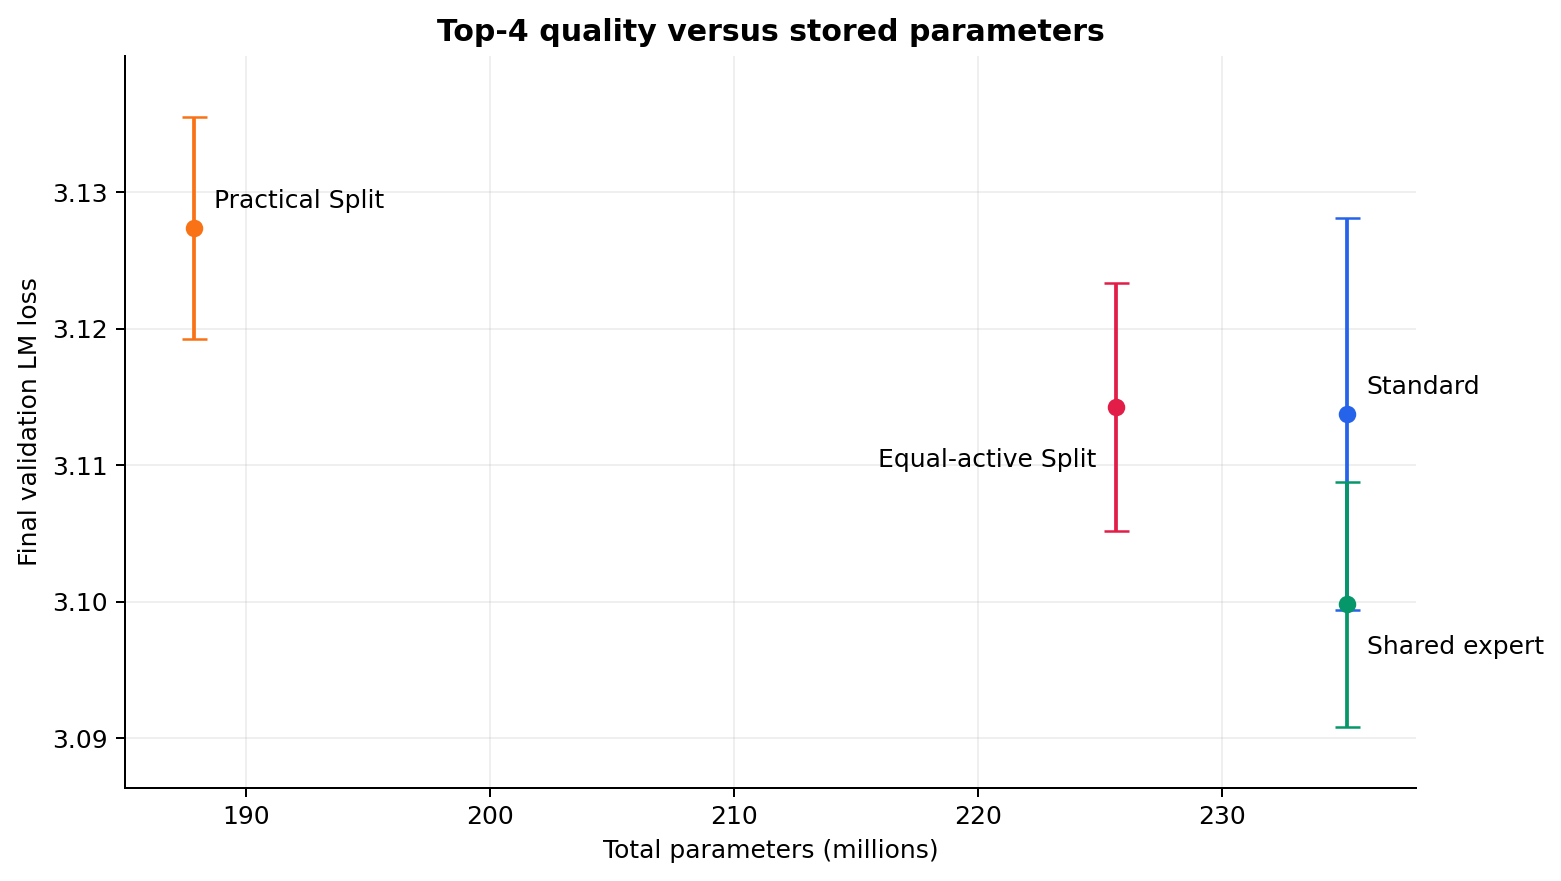
\includegraphics[width=.78\linewidth]{top4_parameter_frontier.png}
\caption{Top-4 quality/storage frontier. Error bars are two-sided 95\% Student's $t$ intervals over three seeds. Matching activated capacity closes the partial-width Split gap; the full shared expert gives the lowest loss at Standard-like storage.}
\label{fig:top4}
\end{figure}

\subsection{External LAMBADA evaluation}
Table~\ref{tab:heldout} reports three-seed means on LAMBADA. The result corroborates the original Top-1 ordering on a separately sourced corpus: Split-25 improves full-token loss in every paired seed. The paired mean difference is $-0.06372$, with 95\% CI $[-0.10240,-0.02504]$. Target-token loss and teacher-forced exact target-sequence rate improve by $-0.34892$ and $+0.01895$; both paired intervals exclude zero. These diagnostics condition on the true preceding tokens and are not free-running generation accuracy. Under Top-4, the full shared expert is numerically better in full-token loss in all seeds, but equal-active Split minus shared is $+0.01019$ $[-0.00762,+0.02801]$ and therefore unresolved.

\begin{table}[t]
\centering
\caption{External LAMBADA evaluation (three-seed means). Exact is teacher-forced target-token sequence match. Training-corpus overlap was not audited.}
\label{tab:heldout}
\begin{tabular}{llrrr}
\hline
Routing & Model & Full loss & Target loss & Exact (\%) \\
\hline
Top-1 & Standard & 4.96044 & 6.88188 & 5.08 \\
Top-1 & Split-25 & \textbf{4.89672} & \textbf{6.53296} & \textbf{6.97} \\
Top-4 & Equal-active Split & 4.77157 & 6.20603 & 8.06 \\
Top-4 & Full shared expert & \textbf{4.76137} & \textbf{6.16261} & \textbf{8.23} \\
\hline
\end{tabular}
\end{table}

\begin{figure}[t]
\centering

\includegraphics[width=.78\linewidth]{top1_lambada.png}
\caption{Top-1 paired external evaluation. Each line connects the same training seed.}
\label{fig:heldout}
\end{figure}

\subsection{Route dependence and expert redundancy}
On five Split-50 checkpoints, normal, wrong-private, shared-only, and private-only losses are 3.141, 3.432, 3.408, and 3.593. Averaging every non-selected alternative, wrong private computation is worse than omitting private computation by 0.02392 $[0.01803,0.02982]$. Corrupting one MoE layer at a time increases loss in every layer and seed, with mean penalties 0.0422, 0.0646, 0.0684, and 0.0478 in layers 2, 4, 6, and 8. Thus private branches are neither inactive nor interchangeable.

We execute every expert on the same sampled hidden states within each checkpoint and measure mean off-diagonal centered cosine and linear CKA \citep{kornblith2019cka}. Width reduction itself lowers similarity, so Standard-512 is the key control. Split private-512 experts have centered cosine 0.0294 versus 0.0850 for Standard-512 (paired difference $-0.05563$ $[-0.06040,-0.05085]$) and CKA 0.3685 versus 0.3949 ($-0.02643$ $[-0.04467,-0.00818]$). This is evidence of lower output redundancy at matched width, not semantic proof that $S$ contains ``common knowledge.''

\begin{figure}[t]
\centering
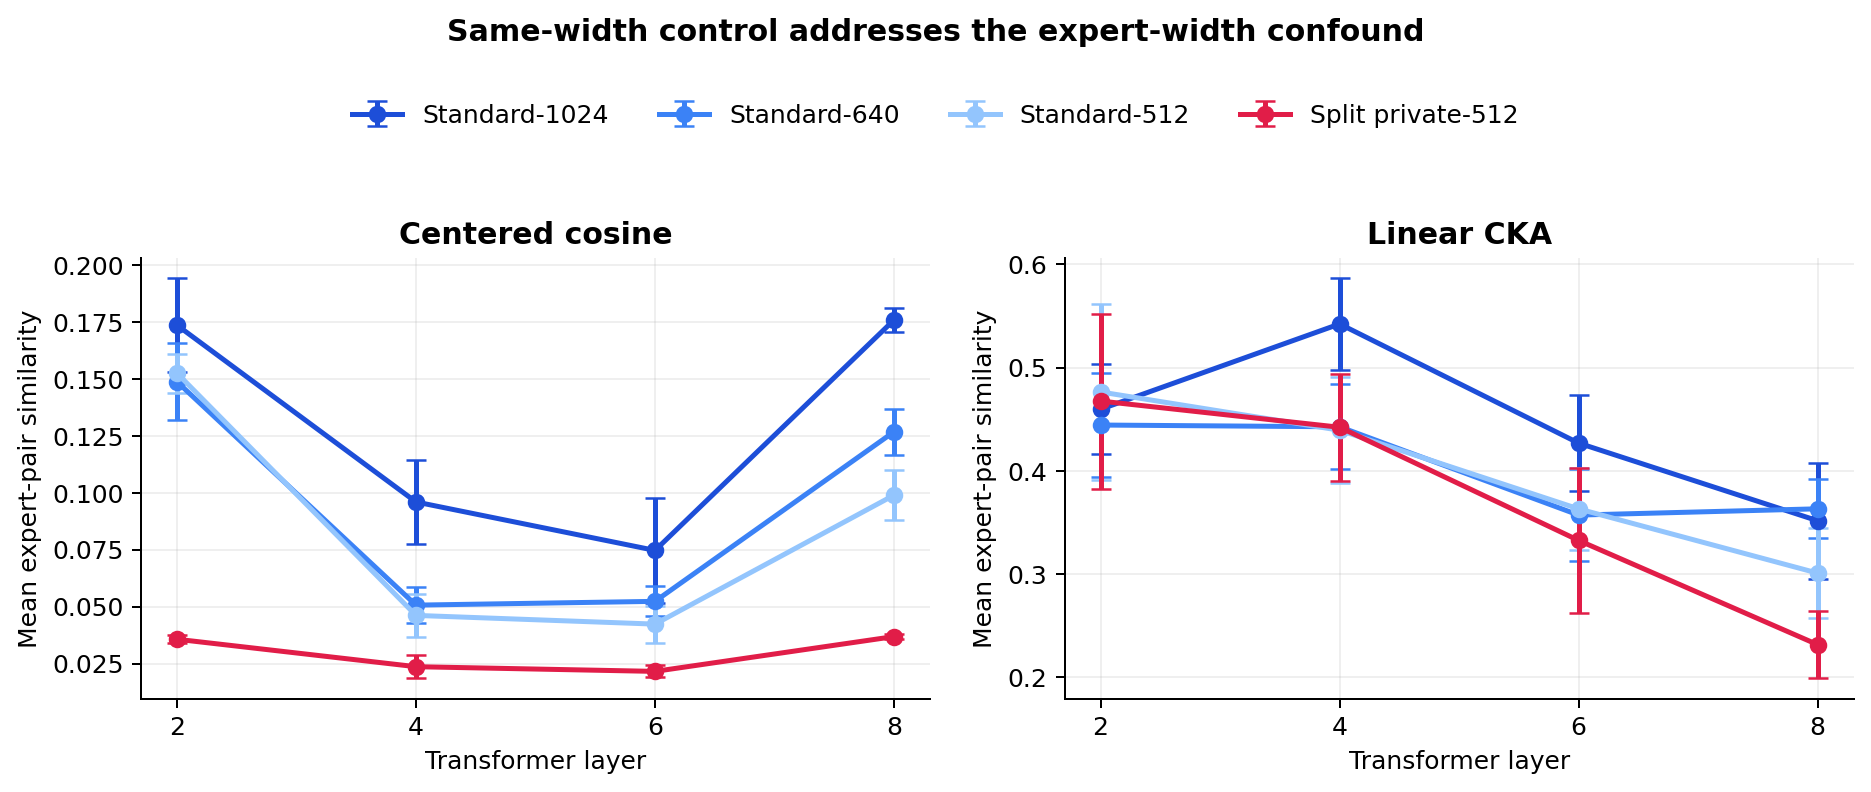
\includegraphics[width=.76\linewidth]{width_controlled_similarity.png}
\caption{Width-controlled expert-output similarity. Error bars are two-sided 95\% Student's $t$ intervals over five seeds. Split private experts remain less similar than conventional experts with the same width.}
\label{fig:similarity}
\end{figure}

\subsection{Systems behavior}
Training throughput does not track activated parameter count exactly because dispatch and launching separate shared/private FFNs carry overhead. Averaged over three logged Top-4 training seeds, practical Split is 2.0\% slower than Standard despite fewer activated parameters, and equal-active Split is 3.0\% slower; practical Split reduces mean peak reserved memory from 6.38 to 5.32 GiB per GPU.

For a SwiGLU FFN, the three projections require approximately $6d_{\mathrm{model}}w$ multiply-add FLOPs per token when one multiply-add counts as two FLOPs. Across eight MoE layers, the Top-1 Standard and Split variants each use approximately 25.17M FFN-projection FLOPs/token. Under Top-4, Standard, equal-active Split, and the full shared expert use approximately 100.66M, while practical Split uses 81.79M. These estimates exclude routing, nonlinearities, attention, embeddings, and the output head; they clarify why activated parameter counts are architectural accounting rather than a runtime measurement.

We additionally run a standardized forward-only benchmark on one Tesla T4, batch 4, context 256, FP16 autocast, ten warmups, and fifty measured iterations. Deterministically initialized weights isolate architecture cost but do not reproduce trained routing distributions. Standard, practical Split, equal-active Split, and the full shared expert reach 19.32k, 17.36k, 18.31k, and 19.44k tokens/s, with peak allocated memory 1.41, 1.16, 1.36, and 1.42 GiB, respectively. The parameter-efficient design saves memory but does not automatically improve throughput in this unfused reference implementation.

\begin{figure}[t]
\centering

\includegraphics[width=.82\linewidth]{standardized_t4.png}
\caption{One-run-per-configuration standardized architecture-only single-T4 benchmark.}
\label{fig:systems}
\end{figure}

\section{Limitations}
The models are small by contemporary language-model standards and use only three confirmatory seeds in the scaling experiments. Initial scaling runs cover 106.5M token positions and the output-scale controls cover 213.0M; neither establishes behavior after large-scale or compute-optimal pretraining. The corpus is a deliberately interpretable four-source mixture rather than a modern trillion-token distribution. Its source revisions were not pinned during original preparation, and it was not deduplicated against LAMBADA, so the external evaluation is not a contamination audit. Only two output scales were tested; Standard's scale sensitivity and the significant architecture-by-scale interaction show that optimization details matter even though Split wins both tested matched comparisons. Top-1 and Top-4 also differ in router weighting, so their effect sizes do not isolate $K$. Confidence intervals with three seeds are wide, and failure to reject a difference is not equivalence. The reference dispatcher is Python-level and unfused; its throughput should not be extrapolated to optimized expert-parallel kernels. Route interventions are out of distribution, and similarity uses each model's native hidden states rather than a cross-model common probe bank. Prior shared-expert and shared-base/delta work limits our contribution to controlled partial-width allocation evidence.

\section{Conclusion}
SplitMoE asks a simple allocation question: should every routed expert independently store its entire FFN transformation? In the tested Top-1 settings, assigning a modest fraction of active width to a shared path improves the observed quality/storage frontier at both tested output scales while preserving route-dependent, less-redundant private experts; external LAMBADA evaluation corroborates the original ordering but is not contamination-audited. Under Top-4 routing, equalizing active capacity closes the partial-width quality gap, but a conventional full shared expert is stronger at matched storage and activation. Shared capacity is useful; the appropriate shared/private granularity depends on routing and systems regime.

\section*{Reproducibility Statement}
The public repository contains model code, exact configurations, pretokenization, paired-seed metrics, intervention and similarity scripts, W\&B exports, and figure-generation scripts. The output-scale protocol was timestamped in repository commit \texttt{60f2f68}; the effective-batch mismatch and corrective cells were recorded before those cells ran in commit \texttt{fa9e55b}. Large checkpoints are not bundled. Configuration and preprocessing code are public, but original training-source revisions were not pinned, so the original pretraining corpus cannot be reconstructed bit-for-bit. LAMBADA and tokenizer revisions, preprocessing, and checksums are recorded in a machine-readable manifest. No optimizer state is required for evaluation.

\bibliographystyle{plainnat}
\bibliography{references}
\end{document}
